% ----------------------------------------------------------
% Capítulo de Resultados
% ----------------------------------------------------------
\chapter{Resultados}
\label{cap:resultados}
% ---

Este capítulo apresenta os resultados da avaliação da plataforma desenvolvida para a Casa de Cultura de João Monlevade, destacando as melhorias na gestão institucional e os impactos positivos que a plataforma trouxe para a automação de processos. Serão discutidos os critérios e métodos de avaliação utilizados, bem como os resultados obtidos em cada um deles.

\section{Critérios de Avaliação}

Os testes e validações da plataforma de artistas monlevadenses foram fundamentados em critérios importantes, que guiaram a avaliação do desempenho geral da plataforma.

\subsection{Funcionalidade} 

O principal objetivo foi verificar se as funcionalidades planejadas, como a publicação de notícias, a exposição dos artistas na "Vitrine", o acompanhamento da Escola de Artes e a divulgação de editais, estavam funcionando corretamente, conforme o escopo do projeto. 

\subsection{Usabilidade} 

Avaliar a facilidade de uso da plataforma foi essencial, levando em consideração a experiência do usuário, a navegabilidade e a acessibilidade. 

\subsection{Desempenho} 

Medimos o tempo de resposta da plataforma sob diferentes cenários de uso, simulando o acesso de um usuário à página principal. A implementação atual do website foi realizada na plataforma PythonAnywhere, utilizando sua categoria gratuita. 

\subsection{Segurança} 
A integridade e proteção dos dados inseridos na plataforma foram rigorosamente avaliadas. O objetivo foi garantir que as informações dos usuários, especialmente dos artistas e administradores, estivessem protegidas contra acessos não autorizados.

\section{Métodos de Avaliação}

Diversos métodos foram aplicados para validar os critérios de avaliação estabelecidos, estes são descritos abaixo.

\subsection{Testes de Funcionalidade} 

Foram realizados testes automatizados utilizando o \textit{framework} Django, focando nas funcionalidades do sistema. Esses testes asseguraram que os modelos e as visualizações do site estivessem operando conforme o esperado. Por exemplo, foi validada a criação de editais, incluindo a verificação se os dados do edital estavam sendo armazenados corretamente e se as visualizações da lista de editais e detalhes estavam acessíveis aos usuários. Além disso, o sistema de inscrição \textit{online} foi testado para garantir que as inscrições fossem processadas corretamente e registradas no banco de dados. Esses testes garantem que a nova funcionalidade não apenas substitui o uso anterior de formulários do Google, mas também otimiza a seleção e organização de eventos culturais, aumentando a eficiência e a transparência das informações.

\subsection{Testes de Usabilidade}

Embora não tenham sido realizados testes de usabilidade com usuários da Casa de Cultura, foram implementados testes automatizados para avaliar a navegabilidade e a funcionalidade do site. Esses testes incluíram a verificação das interações com o formulário de inscrição e com o painel administrativo, garantindo que as principais funcionalidades fossem acessíveis e operacionais. Por exemplo, os testes confirmaram que o formulário de inscrição de artistas estava sendo corretamente exibido e que as informações eram armazenadas no banco de dados, melhorando a gestão dos dados acadêmicos. A abordagem de testar automatizadamente garantiu uma gestão mais organizada e centralizada, permitindo uma análise precisa da funcionalidade do sistema.

\begin{figure}[htb] \caption{\label{fig_grafico}Sucesso nos testes automatizados } \begin{center} 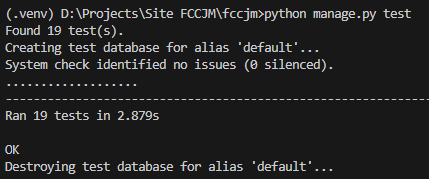
\includegraphics[scale=0.3]{./img/tests.png} \end{center} \legend{Fonte: o autor} \end{figure}

Além disso, foi conduzido um teste utilizando a ferramenta automatizada PageSpeed Insights \cite{PageSpeedInsights}, que graduou o site com notas 100 nos quesitos acessibilidade e uso de práticas recomendadas na categoria de dispositivos móveis, e 97 na categoria Desktop na categoria acessibilidade, com apenas uma consideração sobre o contraste do botão de pesquisa. Esses resultados indicam que o site foi projetado com uma forte ênfase na experiência do usuário, permitindo uma navegação fluida e eficiente em diferentes dispositivos. A pontuação é definida da seguinte forma pela documentação do PageSpeed Insights:

\begin{citacao}
    Na parte superior da seção estão as pontuações de cada categoria, determinadas pela execução do Lighthouse para coletar e analisar informações de diagnóstico sobre a página. Uma pontuação de 90 ou mais é considerado bom. Entre 50 e 89 é uma pontuação que precisa ser melhorada, e abaixo de 50 é considerada ruim. \cite{PageSpeedInsightsDocs}
\end{citacao}

\begin{figure}[htb] \caption{\label{fig_grafico}Avaliação Page Speed Insights} \begin{center} 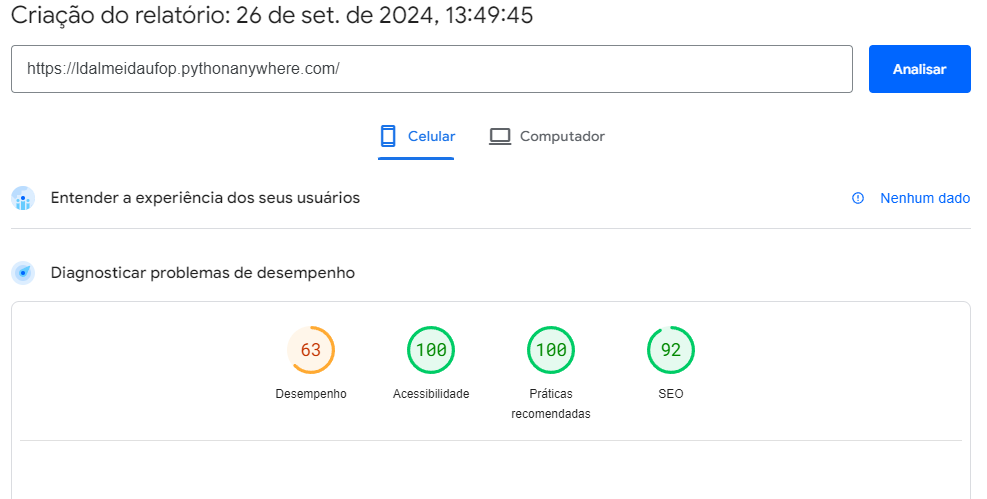
\includegraphics[scale=0.3]{./img/pagespeedinsights.png} \end{center} \legend{Fonte: o autor} \end{figure}

\subsection{Testes de Desempenho}

A escolha de usar um serviço gratuito de hospedagem possibilitou a realização de testes em condições adversas, simulando o pior cenário possível em termos de desempenho, pois os testes foram realizados com a cota de CPU completamente utilizada. Apesar dessas limitações, a plataforma se manteve estável, reforçando seu potencial. Os resultados indicam que, mesmo em condições desfavoráveis, a estrutura da plataforma é robusta e capaz de lidar com a carga de usuários.

Foram utilzadas ferramentas automatizadas de avaliação de sites web. O teste realizado com o GTmetrix \cite{GTMetrix} retornou uma avaliação de 90\% no quesito performance, demonstrando um bom tempo de resposta para o carregamento da página principal. Essa nota reflete a eficiência do código e a adequação das tecnologias utilizadas na construção do site.

\begin{figure}[htb] \caption{\label{fig_grafico}Avaliação GTmetrix} \begin{center} 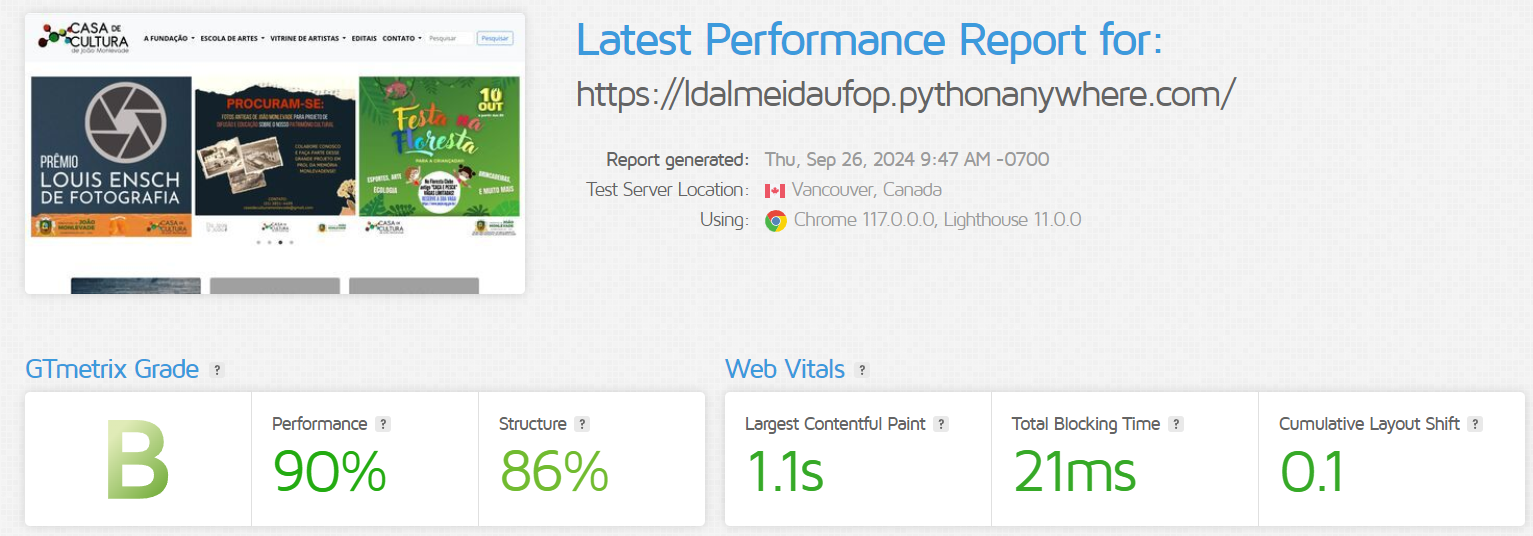
\includegraphics[scale=0.3]{./img/gtmetrix.png} \end{center} \legend{Fonte: o autor} \end{figure}

No entanto, é importante reforçar que esses resultados representam o pior caso. O desempenho da plataforma será consideravelmente melhor quando o site for hospedado pela Prefeitura, que oferecerá mais recursos computacionais e de infraestrutura. Essa migração não só melhorará a velocidade de carregamento, mas também permitirá a implementação de novas funcionalidades que dependem de maior capacidade de processamento.

O código-fonte do site também foi submetido a testes utilizando a ferramenta Validator \cite{Validator}. A partir dela, detectou-se uma oportunidade de melhoria na organização dos \textit{scripts}, como pode ser verificado abaixo. Após a refatoração do código, utilizando as boas práticas e reorganizando a importação dos \textit{scripts}, foi verificada a resolução do problema. Essa etapa de otimização é crucial para garantir a escalabilidade da plataforma, permitindo que ela suporte um aumento no número de usuários sem comprometer o desempenho.

\begin{figure}[htb]
    \label{teste}
    \centering
     \begin{minipage}{0.4\textwidth}
       \centering
       \caption{Erro apontado pelo Validator} \label{fig_minipage_imagem1}
       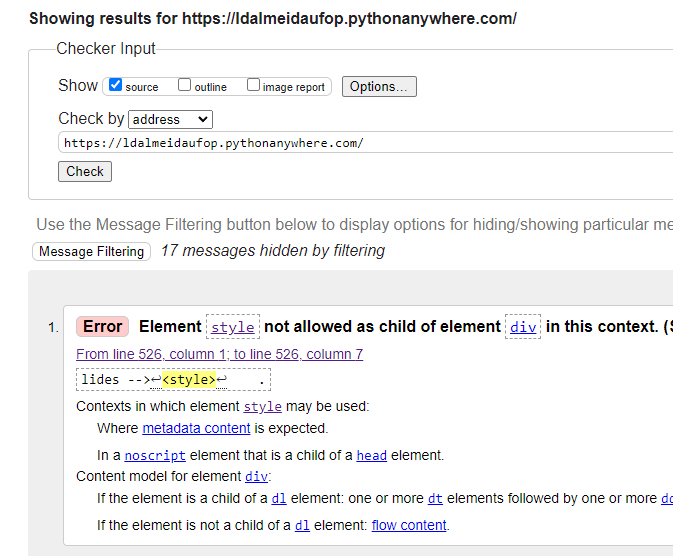
\includegraphics[scale=0.3]{./img/validator_error.png}
       \legend{Fonte: o autor}
     \end{minipage}
     \hfill
     \begin{minipage}{0.4\textwidth}
        \centering
        \caption{Erro corrigido} \label{fig_minipage_imagem2}
        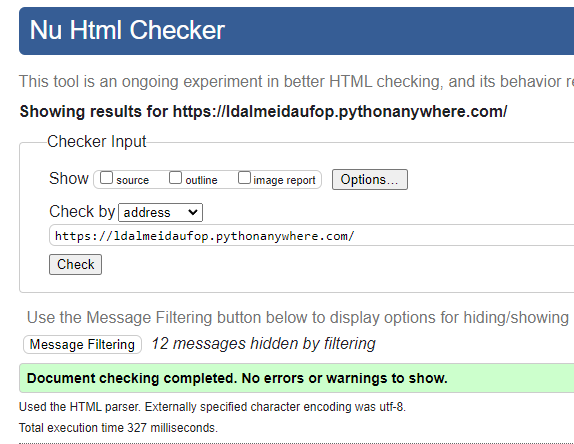
\includegraphics[scale=0.3]{./img/validator_sucess.png}
        \legend{Fonte: o autor}
      \end{minipage}
   \end{figure}

\subsection{Testes de Segurança}

Os \textit{logs} gerados por duas plataformas de teste de segurança \textit{online} foram analizados e ambas não detectaram nenhum risco médio ou grave presente no site, o que demonstra uma preocupação constante com a segurança da informação. O teste realizado pela plataforma Pentest Tools \cite{Pentest} identificou quatro considerações de nível baixo. Essas questões estão relacionadas ao certificado de segurança do site, à falta de ofuscação das tecnologias utilizadas e à visibilidade do arquivo robots.txt, que orienta os \textit{web crawlers} sobre quais \ac{URLs} e \textit{endpoints} da aplicação podem ser acessados.

\begin{figure}[htb] \caption{\label{fig_grafico}Teste do Pentest Tools} \begin{center} 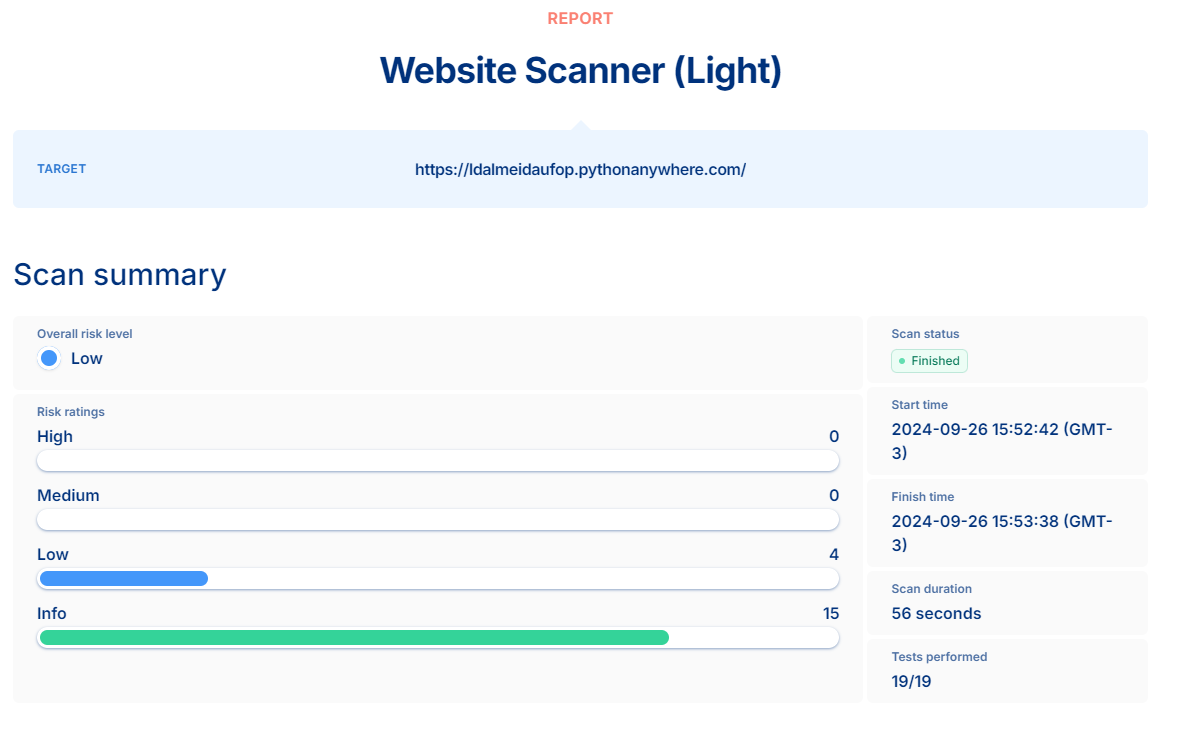
\includegraphics[scale=0.3]{./img/pentest.png} \end{center} \legend{Fonte: o autor} \end{figure}

A outra plataforma utilizada foi a Immuniweb \cite{Immuniweb}. A metodologia de avaliação dessa ferramenta estabelece que o teste começa com uma pontuação de 100, onde pontos são adicionados por configurações boas e confiáveis do site e do servidor web, e pontos são descontados por configurações inseguras, incompletas ou não confiáveis. A pontuação final pode variar de A+ a F, sendo que a nota máxima é A+ e a mínima F. Após a avaliação, o sistema recebeu a nota "A-", indicando um bom nível de segurança. Embora não tenham sido encontradas vulnerabilidades no sistema, foi observado que dois pacotes estavam desatualizados, embora não possuíssem vulnerabilidades conhecidas. Essa avaliação positiva sugere que a plataforma foi projetada e mantida com um foco significativo em práticas de segurança, o que é crucial para proteger os dados sensíveis dos usuários.

\begin{figure}[htb] \caption{\label{fig_grafico}Teste do Immuniweb} \begin{center} 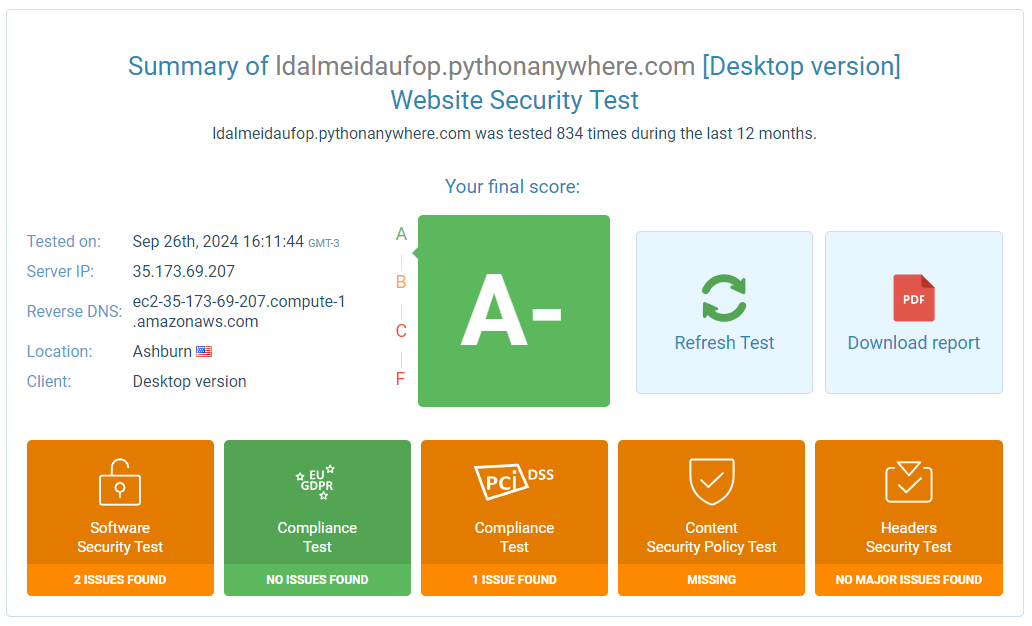
\includegraphics[scale=0.3]{./img/immuniweb.png} \end{center} \legend{Fonte: o autor} \end{figure}

Esses testes de segurança não apenas garantem a integridade da plataforma, mas também reforçam a confiança dos usuários na utilização do sistema. A segurança é um fator crucial, especialmente em plataformas que lidam com dados pessoais e informações acadêmicas, e a adoção de boas práticas de segurança ajudará a manter a credibilidade da Casa de Cultura.

\section{Resultados Obtidos}


Os resultados dos testes automatizados indicam que a plataforma atende aos critérios de funcionalidade estabelecidos no início do projeto. As funcionalidades principais operam corretamente, e os testes demonstraram que a interface é intuitiva e acessível. Em relação ao desempenho, o sistema mostrou-se robusto, respondendo adequadamente aos testes simulados, com apenas pequenos ajustes necessários para otimizar o código-fonte em questões pontuais.

Quanto à segurança, os testes não revelaram vulnerabilidades críticas, e as medidas de proteção dos dados se mostraram eficazes. Porém, será necessário que no momento da implantação do site sejam implementadas rotinas de \textit{backup} automáticas e mecanismos de autenticação robustos ao servidores para garantir a integridade das informações.

Em resumo, a plataforma da Casa de Cultura de João Monlevade se mostrou eficiente nos testes realizados, com bom desempenho, usabilidade adequada e segurança confiável, estando apta a ser utilizada pelos artistas locais e administradores da instituição.